\documentclass[11pt,a4paper]{article}
\usepackage[margin=1in]{geometry}
\usepackage[T1]{fontenc}
\usepackage[utf8]{inputenc}
\usepackage{lmodern}
\usepackage{hyperref}
\usepackage{enumitem}
\usepackage{xurl}
\usepackage{tikz}
\usepackage{float}
\usetikzlibrary{arrows.meta, positioning, shapes.geometric}
\hypersetup{colorlinks=true,linkcolor=blue,urlcolor=blue}
\newcommand{\codepath}[1]{\path{#1}}
\tikzset{
  box/.style={rectangle,draw,rounded corners,align=center,inner sep=3pt,minimum width=44mm},
  decision/.style={diamond,draw,aspect=2.2,align=center,inner sep=2pt},
  line/.style={-Latex}
}

\title{Phase-2 Deliverable: Parameter Sweep Runner}
\author{SIT Engine Documentation}
\date{\today}

\begin{document}
\maketitle

\section{Technical Description}
Sweep runner explores parameter matrices while preserving core SIT schema purity and recording experiment metadata in sweep-specific outputs.

\section{Implementation Fulfillment}
Implemented in \codepath{Phase-2/sweeps/run_param_sweep.py}; visualization handled in \codepath{Phase-2/sweeps/visualize_sweep_results.py}.

\section{Design \& Architecture}
\subsection*{Function Attributes}
\begin{itemize}[leftmargin=*]
  \item \texttt{load\_config()}: Inputs=sweep JSON path; Outputs=parsed config object; Side effects=validates sweep schema and defaults; Failure modes=invalid JSON or missing fields.
  \item \texttt{build\_cases()}: Inputs=matrix dictionary; Outputs=expanded case iterator; Side effects=builds cartesian experiment space; Failure modes=empty matrix, invalid values.
  \item \texttt{to\_cmd()}: Inputs=repo path + case + shared args; Outputs=CLI command list; Side effects=maps config to runnable command; Failure modes=bad target/arg composition.
  \item \texttt{run\_case()}: Inputs=command list + cwd; Outputs=subprocess result; Side effects=executes one sweep case; Failure modes=non-zero return, timeout.
  \item \texttt{main()}: Inputs=CLI args + config; Outputs=summary files + csv; Side effects=orchestrates full sweep lifecycle; Failure modes=partial sweep due to failures.
\end{itemize}
\subsection*{Function Execution Details}
\begin{enumerate}[leftmargin=*]
  \item \texttt{load\_config()}
  \begin{itemize}[leftmargin=*]
    \item Input attributes: sweep JSON path.
    \item Processing flow: validates sweep schema and defaults.
    \item Output attributes: parsed config object.
    \item Failure behavior: invalid JSON or missing fields.
  \end{itemize}
  \item \texttt{build\_cases()}
  \begin{itemize}[leftmargin=*]
    \item Input attributes: matrix dictionary.
    \item Processing flow: builds cartesian experiment space.
    \item Output attributes: expanded case iterator.
    \item Failure behavior: empty matrix, invalid values.
  \end{itemize}
  \item \texttt{to\_cmd()}
  \begin{itemize}[leftmargin=*]
    \item Input attributes: repo path + case + shared args.
    \item Processing flow: maps config to runnable command.
    \item Output attributes: CLI command list.
    \item Failure behavior: bad target/arg composition.
  \end{itemize}
  \item \texttt{run\_case()}
  \begin{itemize}[leftmargin=*]
    \item Input attributes: command list + cwd.
    \item Processing flow: executes one sweep case.
    \item Output attributes: subprocess result.
    \item Failure behavior: non-zero return, timeout.
  \end{itemize}
  \item \texttt{main()}
  \begin{itemize}[leftmargin=*]
    \item Input attributes: CLI args + config.
    \item Processing flow: orchestrates full sweep lifecycle.
    \item Output attributes: summary files + csv.
    \item Failure behavior: partial sweep due to failures.
  \end{itemize}
\end{enumerate}


\subsection*{Diagram A: End-to-End Design Flow}
\begin{figure}[H]
\centering
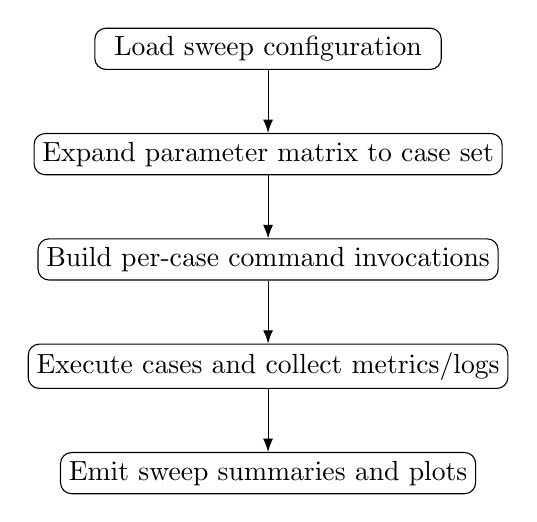
\begin{tikzpicture}[node distance=8mm and 12mm]
\node[box] (a) {Load sweep configuration};
\node[box, below=of a] (b) {Expand parameter matrix to case set};
\node[box, below=of b] (c) {Build per-case command invocations};
\node[box, below=of c] (d) {Execute cases and collect metrics/logs};
\node[box, below=of d] (e) {Emit sweep summaries and plots};
\draw[line] (a) -- (b);
\draw[line] (b) -- (c);
\draw[line] (c) -- (d);
\draw[line] (d) -- (e);
\end{tikzpicture}
\caption{Deliverable 07: End-to-End Design Flow}
\end{figure}

\subsection*{Diagram B: Function Interaction and Attribute Flow}
\begin{figure}[H]
\centering
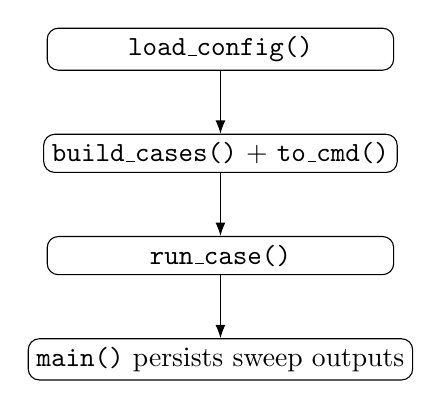
\begin{tikzpicture}[node distance=8mm and 12mm]
\node[box] (fa) {\texttt{load\_config()}};
\node[box, below=of fa] (fb) {\texttt{build\_cases()} + \texttt{to\_cmd()}};
\node[box, below=of fb] (fc) {\texttt{run\_case()}};
\node[box, below=of fc] (fd) {\texttt{main()} persists sweep outputs};
\draw[line] (fa) -- (fb);
\draw[line] (fb) -- (fc);
\draw[line] (fc) -- (fd);
\end{tikzpicture}
\caption{Deliverable 07: Function Interaction and Attribute Flow}
\end{figure}

\end{document}
